\subsection{Synthese}

Für jede Spannungsform sind die Amplituden nach den Formeln aus
\ref{sec:koeffizientenrechnung} so bestimmt worden, dass eine maximale Amplitude
für die erste Oberwelle erreicht wird.

\begin{figure}
  \centering
  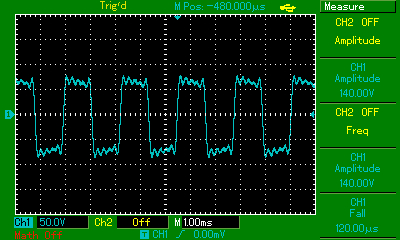
\includegraphics[width=\textwidth]{content/rechteck.jpg}
  \caption{Fourier-Synthese der Rechteckspannung.}
  \label{fig:rechteck}
\end{figure}

\begin{table}
  \centering
  \caption{Synthesewerte der Rechteckspannung.}
  \label{tab:rechtecksynthese}
  \begin{tabular}
    { S[table-format=2.0] S[table-format=3.2] }
    \toprule
    {Oberwelle} & {Amplitude} \\
    \hline
    $\symup{n}$ & $\symup{U}_\text{r} \:/\: \si{\volt}$ \\
    \midrule
     1 & 179.50 \\
     2 &  89.50 \\
     3 &  59.80 \\
     4 &  44.75 \\
     5 &  35.84 \\
     6 &  29.90 \\
     7 &  25.54 \\
     8 &  22.37 \\
     9 &  19.80 \\
    10 &  18.02 \\
    \bottomrule
  \end{tabular}
\end{table}

\begin{figure}
  \centering
  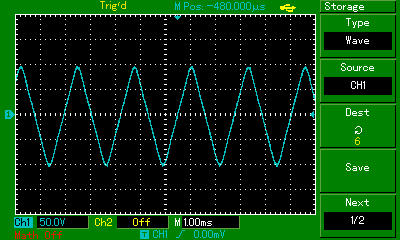
\includegraphics[width=\textwidth]{content/dreieck.jpg}
  \caption{Fourier-Synthese der Dreieckspannung.}
  \label{fig:dreieck}
\end{figure}

\begin{table}
  \centering
  \caption{Synthesewerte der Dreieckspannung.}
  \label{tab:dreieckwerte}
  \begin{tabular}
    { S[table-format=1.0] S[table-format=3.2] }
    \toprule
    {Oberwelle} & {Amplitude} \\
    \hline
    $\symup{n}$ & $\symup{U}_\text{d} \:/\: \si{\volt}$ \\
    \midrule
    1 & 179.30 \\
    3 &  20.00 \\
    5 &   7.00 \\
    \bottomrule
  \end{tabular}
\end{table}

\begin{figure}
  \centering
  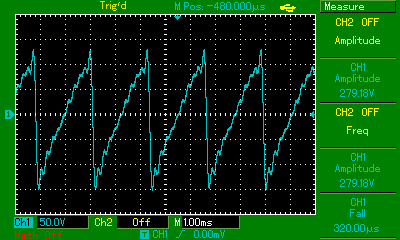
\includegraphics[width=\textwidth]{content/saegezahn.jpg}
  \caption{Fourier-Synthese der Sägezahnspannung.}
  \label{fig:saege}
\end{figure}

\begin{table}
  \centering
  \caption{Synthesewerte der Sägezahnspannung.}
  \label{tab:saegewerte}
  \begin{tabular}
    { S[table-format=2.0] S[table-format=3.2] }
    \toprule
    {Oberwelle} & {Amplitude} \\
    \hline
    $\symup{n}$ & $\symup{U}_\text{s} \:/\: \si{\volt}$ \\
    \midrule
     1 & 179.50 \\
     2 &  89.50 \\
     3 &  60.00 \\
     4 &  45.00 \\
     5 &  35.80 \\
     6 &  30.10 \\
     7 &  25.50 \\
     8 &  22.30 \\
     9 &  20.00 \\
    10 &  18.00 \\
    \bottomrule
  \end{tabular}
\end{table}

\newpage
